

\tikzset{every picture/.style={line width=0.75pt}} %set default line width to 0.75pt        

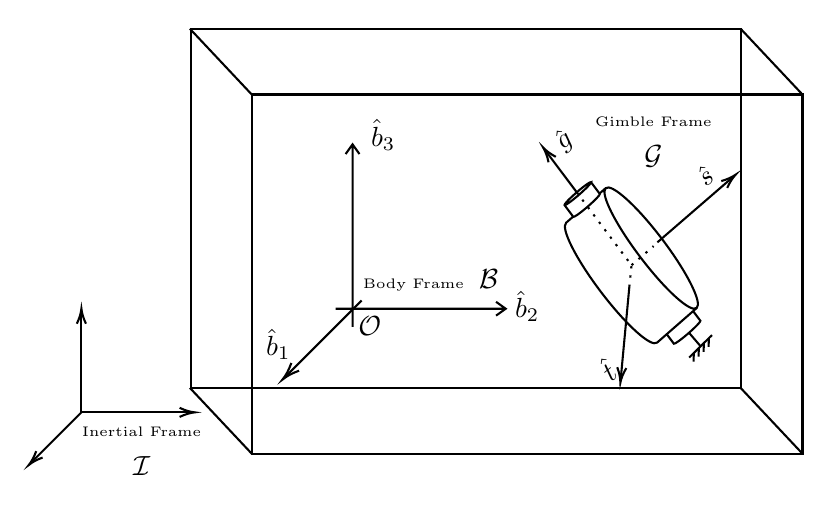
\begin{tikzpicture}[x=0.5pt,y=0.5pt,yscale=-1,xscale=1]
%uncomment if require: \path (0,350); %set diagram left start at 0, and has height of 350

%Shape: Can [id:dp8331189729524409] 
\draw  [fill={rgb, 255:red, 255; green, 255; blue, 255 }  ,fill opacity=1 ] (495.82,215.43) -- (502.2,223.92) .. controls (502.6,224.46) and (498.63,228.59) .. (493.34,233.17) .. controls (488.05,237.74) and (483.44,241.02) .. (483.04,240.49) -- (476.66,231.99) .. controls (476.26,231.46) and (480.23,227.32) .. (485.52,222.75) .. controls (490.81,218.17) and (495.42,214.9) .. (495.82,215.43) .. controls (496.22,215.96) and (492.25,220.1) .. (486.97,224.67) .. controls (481.68,229.25) and (477.06,232.52) .. (476.66,231.99) ;
%Shape: Can [id:dp8805062966141313] 
\draw  [color={rgb, 255:red, 0; green, 0; blue, 0 }  ,draw opacity=1 ][fill={rgb, 255:red, 255; green, 255; blue, 255 }  ,fill opacity=1 ] (499.54,214.7) -- (470.96,239.69) .. controls (466.71,243.41) and (448.54,227.03) .. (430.38,203.12) .. controls (412.22,179.2) and (400.94,156.79) .. (405.19,153.08) -- (433.77,128.08) .. controls (438.02,124.37) and (456.19,140.74) .. (474.35,164.66) .. controls (492.51,188.58) and (503.79,210.99) .. (499.54,214.7) .. controls (495.29,218.42) and (477.12,202.04) .. (458.96,178.12) .. controls (440.79,154.21) and (429.52,131.8) .. (433.77,128.08) ;
%Shape: Can [id:dp6975809963098918] 
\draw  [fill={rgb, 255:red, 255; green, 255; blue, 255 }  ,fill opacity=1 ] (423.17,123.76) -- (429.54,132.26) .. controls (429.94,132.79) and (425.98,136.93) .. (420.69,141.5) .. controls (415.4,146.07) and (410.79,149.35) .. (410.39,148.82) -- (404.01,140.32) .. controls (403.61,139.79) and (407.58,135.65) .. (412.86,131.08) .. controls (418.15,126.5) and (422.77,123.23) .. (423.17,123.76) .. controls (423.57,124.29) and (419.6,128.43) .. (414.31,133.01) .. controls (409.02,137.58) and (404.41,140.86) .. (404.01,140.32) ;
%Straight Lines [id:da7548151699735375] 
\draw  [dash pattern={on 0.84pt off 2.51pt}]  (450.87,199.43) -- (452.44,183.78) ;
%Straight Lines [id:da4676995296398143] 
\draw  [dash pattern={on 0.84pt off 2.51pt}]  (452.44,183.78) -- (468.4,169.98) ;
%Straight Lines [id:da24364084418605625] 
\draw  [dash pattern={on 0.84pt off 2.51pt}]  (412.86,131.08) -- (452.44,183.78) ;
%Straight Lines [id:da603601196492777] 
\draw    (471.13,167.25) -- (526.21,119.62) ;
\draw [shift={(527.73,118.31)}, rotate = 499.15] [color={rgb, 255:red, 0; green, 0; blue, 0 }  ][line width=0.75]    (10.93,-3.29) .. controls (6.95,-1.4) and (3.31,-0.3) .. (0,0) .. controls (3.31,0.3) and (6.95,1.4) .. (10.93,3.29)   ;
%Straight Lines [id:da39680954875025143] 
\draw    (450.87,199.43) -- (444.58,266.71) ;
\draw [shift={(444.39,268.7)}, rotate = 275.34000000000003] [color={rgb, 255:red, 0; green, 0; blue, 0 }  ][line width=0.75]    (10.93,-3.29) .. controls (6.95,-1.4) and (3.31,-0.3) .. (0,0) .. controls (3.31,0.3) and (6.95,1.4) .. (10.93,3.29)   ;
%Straight Lines [id:da931335338150046] 
\draw    (412.86,131.08) -- (389.74,100.28) ;
\draw [shift={(388.54,98.68)}, rotate = 413.1] [color={rgb, 255:red, 0; green, 0; blue, 0 }  ][line width=0.75]    (10.93,-3.29) .. controls (6.95,-1.4) and (3.31,-0.3) .. (0,0) .. controls (3.31,0.3) and (6.95,1.4) .. (10.93,3.29)   ;
%Straight Lines [id:da06748543672273133] 
\draw    (510.61,234.25) -- (494.14,250.49) ;
%Straight Lines [id:da33848315956607067] 
\draw    (493.86,232.43) -- (502.38,242.37) ;
%Straight Lines [id:da9582167503794932] 
\draw    (501.06,243.67) -- (500.93,249.9) ;
%Straight Lines [id:da1212417766847036] 
\draw    (497.44,247.24) -- (497.31,253.48) ;
%Straight Lines [id:da09420728047826432] 
\draw    (508.3,236.52) -- (508.18,242.76) ;
%Straight Lines [id:da8325536037855037] 
\draw    (504.68,240.09) -- (504.56,246.33) ;


%Shape: Rectangle [id:dp2711095269864183] 
\draw   (134,12.86) -- (531.27,12.86) -- (531.27,272.43) -- (134,272.43) -- cycle ;
%Shape: Rectangle [id:dp9597125724935636] 
\draw   (178,60.43) -- (576,60.43) -- (576,320) -- (178,320) -- cycle ;
%Straight Lines [id:da6047312216963134] 
\draw    (133.27,12.86) -- (178,60.43) ;
%Straight Lines [id:da614844554115443] 
\draw    (531.27,12.86) -- (576,60.43) ;
%Straight Lines [id:da9657702374196164] 
\draw    (133.27,272.43) -- (178,320) ;
%Straight Lines [id:da4943938352124151] 
\draw    (531.27,272.43) -- (576,320) ;
%Shape: Axis 2D [id:dp8483204934107569] 
\draw  (238.54,215.23) -- (361.54,215.23)(250.84,96.43) -- (250.84,228.43) (354.54,210.23) -- (361.54,215.23) -- (354.54,220.23) (245.84,103.43) -- (250.84,96.43) -- (255.84,103.43)  ;
%Straight Lines [id:da10965728905002736] 
\draw    (257.39,209.23) -- (201.53,265.09) ;
\draw [shift={(200.12,266.5)}, rotate = 315] [color={rgb, 255:red, 0; green, 0; blue, 0 }  ][line width=0.75]    (13.12,-3.95) .. controls (8.34,-1.68) and (3.97,-0.36) .. (0,0) .. controls (3.97,0.36) and (8.34,1.68) .. (13.12,3.95)   ;
%Straight Lines [id:da6362005944191291] 
\draw    (54.88,290.12) -- (18.21,326.79) ;
\draw [shift={(16.8,328.2)}, rotate = 315] [color={rgb, 255:red, 0; green, 0; blue, 0 }  ][line width=0.75]    (10.93,-3.29) .. controls (6.95,-1.4) and (3.31,-0.3) .. (0,0) .. controls (3.31,0.3) and (6.95,1.4) .. (10.93,3.29)   ;
%Straight Lines [id:da9762169812039505] 
\draw    (54.88,290.12) -- (134.8,290.12) ;
\draw [shift={(136.8,290.12)}, rotate = 180] [color={rgb, 255:red, 0; green, 0; blue, 0 }  ][line width=0.75]    (10.93,-3.29) .. controls (6.95,-1.4) and (3.31,-0.3) .. (0,0) .. controls (3.31,0.3) and (6.95,1.4) .. (10.93,3.29)   ;
%Straight Lines [id:da8439523067648185] 
\draw    (54.88,290.12) -- (54.88,217.11) ;
\draw [shift={(54.88,215.11)}, rotate = 450] [color={rgb, 255:red, 0; green, 0; blue, 0 }  ][line width=0.75]    (10.93,-3.29) .. controls (6.95,-1.4) and (3.31,-0.3) .. (0,0) .. controls (3.31,0.3) and (6.95,1.4) .. (10.93,3.29)   ;

% Text Node
\draw (459.47,94.83) node [anchor=north west][inner sep=0.75pt]    {$\mathcal{G} $};
% Text Node
\draw (423.88,74.43) node [anchor=north west][inner sep=0.75pt]   [align=left] {{\selectfont {\tiny Gimble Frame}}};
% Text Node
\draw (256.21,191.43) node [anchor=north west][inner sep=0.75pt]   [align=left] {{\selectfont {\tiny Body Frame}}};
% Text Node
\draw (186.18,227.83) node [anchor=north west][inner sep=0.75pt]    {$\hat{b}_{1}$};
% Text Node
\draw (366,200.4) node [anchor=north west][inner sep=0.75pt]    {$\hat{b}_{2}$};
% Text Node
\draw (262,76.4) node [anchor=north west][inner sep=0.75pt]    {$\hat{b}_{3}$};
% Text Node
\draw (340,185.0) node [anchor=north west][inner sep=0.75pt]    {$\mathcal{B} $};
% Text Node
\draw (494.35,116.24) node [anchor=north west][inner sep=0.75pt]  [rotate=-321.14]  {$\hat{s}$};
% Text Node
\draw (390.94,90.08) node [anchor=north west][inner sep=0.75pt]  [rotate=-321.14]  {$\hat{g}$};
% Text Node
\draw (423.5,254.57) node [anchor=north west][inner sep=0.75pt]  [rotate=-321.14]  {$\hat{t}$};
% Text Node
\draw (252.84,218.63) node [anchor=north west][inner sep=0.75pt]    {$\mathcal{O} $};
% Text Node
\draw (53.21,298.43) node [anchor=north west][inner sep=0.75pt]   [align=left] {{\selectfont {\tiny Inertial Frame}}};
% Text Node
\draw (90,320) node [anchor=north west][inner sep=0.75pt]    {$\mathcal{I} $};

\end{tikzpicture}
